% !TEX encoding = UTF-8 Unicode
\documentclass[10pt]{standalone}\usepackage{tikz,graphicx}
\usepackage{fontspec}
\setmainfont{Arial}
\setsansfont{Arial}\begin{document}

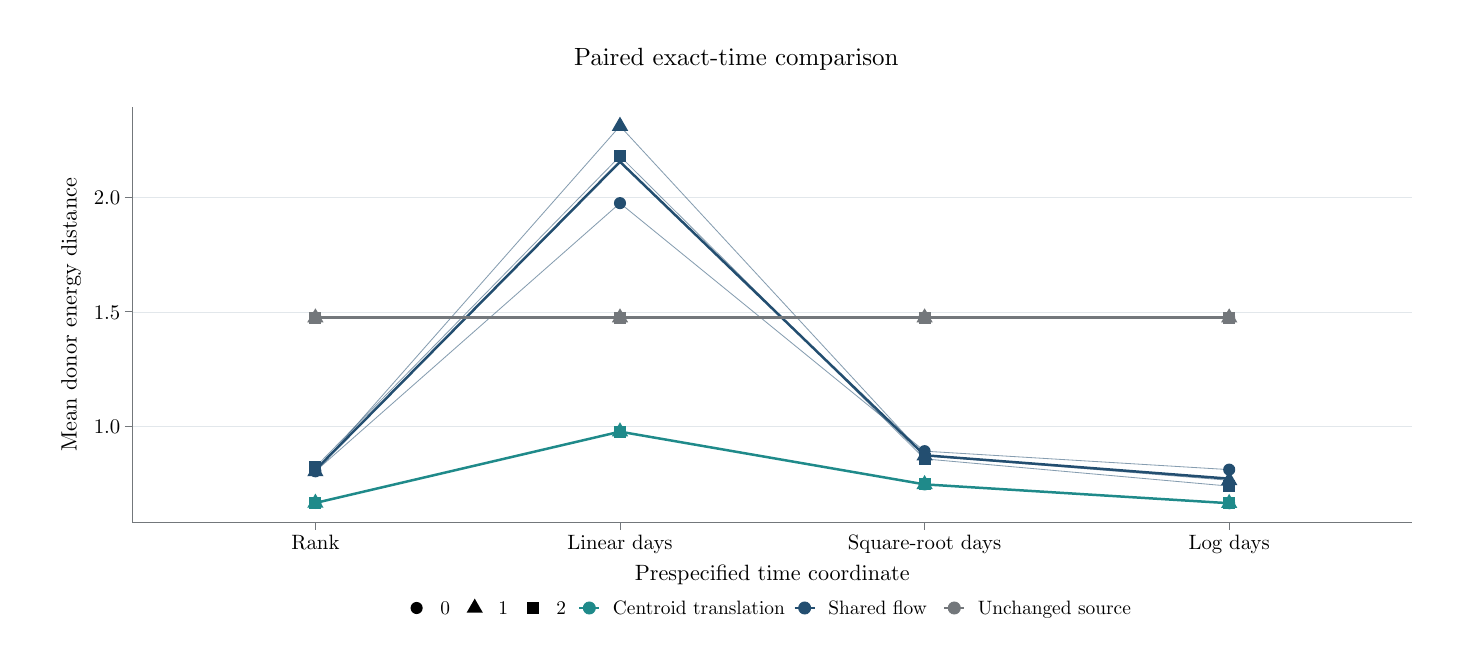
\begin{tikzpicture}[x=1pt,y=1pt]
\definecolor{fillColor}{RGB}{255,255,255}
\path[use as bounding box,fill=fillColor,fill opacity=0.00] (0,0) rectangle (512.15,221.93);
\begin{scope}
\path[clip] (  0.00,  0.00) rectangle (512.15,221.93);
\definecolor{drawColor}{RGB}{0,0,0}

\node[text=drawColor,anchor=base,inner sep=0pt, outer sep=0pt, scale=  0.90] at (256.07,208.38) {Paired exact-time comparison};
\end{scope}
\begin{scope}
\path[clip] (  8.54,  4.27) rectangle (503.61,198.32);
\definecolor{fillColor}{RGB}{255,255,255}

\path[fill=fillColor] (  8.54,  4.27) rectangle (503.61,198.32);
\end{scope}
\begin{scope}
\path[clip] ( 37.93, 43.27) rectangle (500.20,193.19);
\definecolor{fillColor}{RGB}{255,255,255}

\path[fill=fillColor] ( 37.93, 43.27) rectangle (500.20,193.19);
\definecolor{drawColor}{RGB}{226,231,235}

\path[draw=drawColor,line width= 0.2pt,line join=round] ( 37.93, 77.81) --
	(500.20, 77.81);

\path[draw=drawColor,line width= 0.2pt,line join=round] ( 37.93,119.25) --
	(500.20,119.25);

\path[draw=drawColor,line width= 0.2pt,line join=round] ( 37.93,160.69) --
	(500.20,160.69);
\definecolor{drawColor}{RGB}{31,138,138}

\path[draw=drawColor,draw opacity=0.55,line width= 0.3pt,line join=round] (103.97, 50.19) --
	(214.03, 75.95) --
	(324.10, 56.90) --
	(434.16, 50.09);
\definecolor{drawColor}{RGB}{35,78,112}

\path[draw=drawColor,draw opacity=0.55,line width= 0.3pt,line join=round] (103.97, 61.62) --
	(214.03,158.53) --
	(324.10, 68.90) --
	(434.16, 62.23);
\definecolor{drawColor}{RGB}{115,119,123}

\path[draw=drawColor,draw opacity=0.55,line width= 0.3pt,line join=round] (103.97,117.14) --
	(214.03,117.14) --
	(324.10,117.14) --
	(434.16,117.14);
\definecolor{drawColor}{RGB}{31,138,138}

\path[draw=drawColor,draw opacity=0.55,line width= 0.3pt,line join=round] (103.97, 50.19) --
	(214.03, 75.95) --
	(324.10, 56.90) --
	(434.16, 50.09);
\definecolor{drawColor}{RGB}{35,78,112}

\path[draw=drawColor,draw opacity=0.55,line width= 0.3pt,line join=round] (103.97, 61.55) --
	(214.03,186.38) --
	(324.10, 67.26) --
	(434.16, 58.37);
\definecolor{drawColor}{RGB}{115,119,123}

\path[draw=drawColor,draw opacity=0.55,line width= 0.3pt,line join=round] (103.97,117.14) --
	(214.03,117.14) --
	(324.10,117.14) --
	(434.16,117.14);
\definecolor{drawColor}{RGB}{31,138,138}

\path[draw=drawColor,draw opacity=0.55,line width= 0.3pt,line join=round] (103.97, 50.19) --
	(214.03, 75.95) --
	(324.10, 56.90) --
	(434.16, 50.09);
\definecolor{drawColor}{RGB}{35,78,112}

\path[draw=drawColor,draw opacity=0.55,line width= 0.3pt,line join=round] (103.97, 63.14) --
	(214.03,175.49) --
	(324.10, 66.11) --
	(434.16, 56.27);
\definecolor{drawColor}{RGB}{115,119,123}

\path[draw=drawColor,draw opacity=0.55,line width= 0.3pt,line join=round] (103.97,117.14) --
	(214.03,117.14) --
	(324.10,117.14) --
	(434.16,117.14);
\definecolor{fillColor}{RGB}{35,78,112}

\path[fill=fillColor] (214.03,158.53) circle (  2.19);

\path[fill=fillColor] (434.16, 62.23) circle (  2.19);

\path[fill=fillColor] (103.97, 61.62) circle (  2.19);

\path[fill=fillColor] (324.10, 68.90) circle (  2.19);

\path[fill=fillColor] (214.03,189.78) --
	(216.98,184.68) --
	(211.09,184.68) --
	cycle;

\path[fill=fillColor] (434.16, 61.77) --
	(437.11, 56.67) --
	(431.22, 56.67) --
	cycle;

\path[fill=fillColor] (103.97, 64.95) --
	(106.91, 59.85) --
	(101.02, 59.85) --
	cycle;

\path[fill=fillColor] (324.10, 70.66) --
	(327.04, 65.56) --
	(321.15, 65.56) --
	cycle;

\path[fill=fillColor] (211.85,173.30) --
	(216.22,173.30) --
	(216.22,177.68) --
	(211.85,177.68) --
	cycle;

\path[fill=fillColor] (431.97, 54.08) --
	(436.35, 54.08) --
	(436.35, 58.46) --
	(431.97, 58.46) --
	cycle;

\path[fill=fillColor] (101.78, 60.95) --
	(106.16, 60.95) --
	(106.16, 65.32) --
	(101.78, 65.32) --
	cycle;

\path[fill=fillColor] (321.91, 63.93) --
	(326.28, 63.93) --
	(326.28, 68.30) --
	(321.91, 68.30) --
	cycle;
\definecolor{fillColor}{RGB}{31,138,138}

\path[fill=fillColor] (214.03, 75.95) circle (  2.19);

\path[fill=fillColor] (434.16, 50.09) circle (  2.19);

\path[fill=fillColor] (103.97, 50.19) circle (  2.19);

\path[fill=fillColor] (324.10, 56.90) circle (  2.19);

\path[fill=fillColor] (214.03, 79.35) --
	(216.98, 74.25) --
	(211.09, 74.25) --
	cycle;

\path[fill=fillColor] (434.16, 53.49) --
	(437.11, 48.39) --
	(431.22, 48.39) --
	cycle;

\path[fill=fillColor] (103.97, 53.59) --
	(106.91, 48.49) --
	(101.02, 48.49) --
	cycle;

\path[fill=fillColor] (324.10, 60.30) --
	(327.04, 55.20) --
	(321.15, 55.20) --
	cycle;

\path[fill=fillColor] (211.85, 73.76) --
	(216.22, 73.76) --
	(216.22, 78.13) --
	(211.85, 78.13) --
	cycle;

\path[fill=fillColor] (431.97, 47.90) --
	(436.35, 47.90) --
	(436.35, 52.27) --
	(431.97, 52.27) --
	cycle;

\path[fill=fillColor] (101.78, 48.01) --
	(106.16, 48.01) --
	(106.16, 52.38) --
	(101.78, 52.38) --
	cycle;

\path[fill=fillColor] (321.91, 54.71) --
	(326.28, 54.71) --
	(326.28, 59.09) --
	(321.91, 59.09) --
	cycle;
\definecolor{fillColor}{RGB}{115,119,123}

\path[fill=fillColor] (214.03,117.14) circle (  2.19);

\path[fill=fillColor] (434.16,117.14) circle (  2.19);

\path[fill=fillColor] (103.97,117.14) circle (  2.19);

\path[fill=fillColor] (324.10,117.14) circle (  2.19);

\path[fill=fillColor] (214.03,120.54) --
	(216.98,115.44) --
	(211.09,115.44) --
	cycle;

\path[fill=fillColor] (434.16,120.54) --
	(437.11,115.44) --
	(431.22,115.44) --
	cycle;

\path[fill=fillColor] (103.97,120.54) --
	(106.91,115.44) --
	(101.02,115.44) --
	cycle;

\path[fill=fillColor] (324.10,120.54) --
	(327.04,115.44) --
	(321.15,115.44) --
	cycle;

\path[fill=fillColor] (211.85,114.96) --
	(216.22,114.96) --
	(216.22,119.33) --
	(211.85,119.33) --
	cycle;

\path[fill=fillColor] (431.97,114.96) --
	(436.35,114.96) --
	(436.35,119.33) --
	(431.97,119.33) --
	cycle;

\path[fill=fillColor] (101.78,114.96) --
	(106.16,114.96) --
	(106.16,119.33) --
	(101.78,119.33) --
	cycle;

\path[fill=fillColor] (321.91,114.96) --
	(326.28,114.96) --
	(326.28,119.33) --
	(321.91,119.33) --
	cycle;
\definecolor{drawColor}{RGB}{31,138,138}

\path[draw=drawColor,line width= 0.9pt,line join=round] (103.97, 50.19) --
	(214.03, 75.95) --
	(324.10, 56.90) --
	(434.16, 50.09);
\definecolor{drawColor}{RGB}{35,78,112}

\path[draw=drawColor,line width= 0.9pt,line join=round] (103.97, 62.10) --
	(214.03,173.47) --
	(324.10, 67.42) --
	(434.16, 58.96);
\definecolor{drawColor}{RGB}{115,119,123}

\path[draw=drawColor,line width= 0.9pt,line join=round] (103.97,117.14) --
	(214.03,117.14) --
	(324.10,117.14) --
	(434.16,117.14);
\end{scope}
\begin{scope}
\path[clip] (  0.00,  0.00) rectangle (512.15,221.93);
\definecolor{drawColor}{RGB}{115,119,123}

\path[draw=drawColor,line width= 0.3pt,line join=round,line cap=rect] ( 37.93, 43.27) --
	( 37.93,193.19);
\end{scope}
\begin{scope}
\path[clip] (  0.00,  0.00) rectangle (512.15,221.93);
\definecolor{drawColor}{RGB}{0,0,0}

\node[text=drawColor,anchor=base east,inner sep=0pt, outer sep=0pt, scale=  0.75] at ( 33.49, 75.13) {1.0};

\node[text=drawColor,anchor=base east,inner sep=0pt, outer sep=0pt, scale=  0.75] at ( 33.49,116.57) {1.5};

\node[text=drawColor,anchor=base east,inner sep=0pt, outer sep=0pt, scale=  0.75] at ( 33.49,158.00) {2.0};
\end{scope}
\begin{scope}
\path[clip] (  0.00,  0.00) rectangle (512.15,221.93);
\definecolor{drawColor}{RGB}{115,119,123}

\path[draw=drawColor,line width= 0.3pt,line join=round] ( 35.09, 77.81) --
	( 37.93, 77.81);

\path[draw=drawColor,line width= 0.3pt,line join=round] ( 35.09,119.25) --
	( 37.93,119.25);

\path[draw=drawColor,line width= 0.3pt,line join=round] ( 35.09,160.69) --
	( 37.93,160.69);
\end{scope}
\begin{scope}
\path[clip] (  0.00,  0.00) rectangle (512.15,221.93);
\definecolor{drawColor}{RGB}{115,119,123}

\path[draw=drawColor,line width= 0.3pt,line join=round,line cap=rect] ( 37.93, 43.27) --
	(500.20, 43.27);
\end{scope}
\begin{scope}
\path[clip] (  0.00,  0.00) rectangle (512.15,221.93);
\definecolor{drawColor}{RGB}{115,119,123}

\path[draw=drawColor,line width= 0.3pt,line join=round] (103.97, 40.43) --
	(103.97, 43.27);

\path[draw=drawColor,line width= 0.3pt,line join=round] (214.03, 40.43) --
	(214.03, 43.27);

\path[draw=drawColor,line width= 0.3pt,line join=round] (324.10, 40.43) --
	(324.10, 43.27);

\path[draw=drawColor,line width= 0.3pt,line join=round] (434.16, 40.43) --
	(434.16, 43.27);
\end{scope}
\begin{scope}
\path[clip] (  0.00,  0.00) rectangle (512.15,221.93);
\definecolor{drawColor}{RGB}{0,0,0}

\node[text=drawColor,anchor=base,inner sep=0pt, outer sep=0pt, scale=  0.75] at (103.97, 33.46) {Rank};

\node[text=drawColor,anchor=base,inner sep=0pt, outer sep=0pt, scale=  0.75] at (214.03, 33.46) {Linear days};

\node[text=drawColor,anchor=base,inner sep=0pt, outer sep=0pt, scale=  0.75] at (324.10, 33.46) {Square-root days};

\node[text=drawColor,anchor=base,inner sep=0pt, outer sep=0pt, scale=  0.75] at (434.16, 33.46) {Log days};
\end{scope}
\begin{scope}
\path[clip] (  0.00,  0.00) rectangle (512.15,221.93);
\definecolor{drawColor}{RGB}{0,0,0}

\node[text=drawColor,anchor=base,inner sep=0pt, outer sep=0pt, scale=  0.80] at (269.06, 22.17) {Prespecified time coordinate};
\end{scope}
\begin{scope}
\path[clip] (  0.00,  0.00) rectangle (512.15,221.93);
\definecolor{drawColor}{RGB}{0,0,0}

\node[text=drawColor,rotate= 90.00,anchor=base,inner sep=0pt, outer sep=0pt, scale=  0.80] at ( 17.68,118.23) {Mean donor energy distance};
\end{scope}
\begin{scope}
\path[clip] (  0.00,  0.00) rectangle (512.15,221.93);
\definecolor{fillColor}{RGB}{255,255,255}

\path[fill=fillColor] (135.99,  7.68) rectangle (194.98, 16.79);
\end{scope}
\begin{scope}
\path[clip] (  0.00,  0.00) rectangle (512.15,221.93);
\definecolor{fillColor}{RGB}{255,255,255}

\path[fill=fillColor] (135.99,  7.68) rectangle (145.10, 16.79);
\definecolor{fillColor}{RGB}{0,0,0}

\path[fill=fillColor] (140.54, 12.23) circle (  2.19);
\end{scope}
\begin{scope}
\path[clip] (  0.00,  0.00) rectangle (512.15,221.93);
\definecolor{fillColor}{RGB}{255,255,255}

\path[fill=fillColor] (156.99,  7.68) rectangle (166.09, 16.79);
\definecolor{fillColor}{RGB}{0,0,0}

\path[fill=fillColor] (161.54, 15.63) --
	(164.49, 10.53) --
	(158.60, 10.53) --
	cycle;
\end{scope}
\begin{scope}
\path[clip] (  0.00,  0.00) rectangle (512.15,221.93);
\definecolor{fillColor}{RGB}{255,255,255}

\path[fill=fillColor] (177.99,  7.68) rectangle (187.09, 16.79);
\definecolor{fillColor}{RGB}{0,0,0}

\path[fill=fillColor] (180.35, 10.05) --
	(184.73, 10.05) --
	(184.73, 14.42) --
	(180.35, 14.42) --
	cycle;
\end{scope}
\begin{scope}
\path[clip] (  0.00,  0.00) rectangle (512.15,221.93);
\definecolor{drawColor}{RGB}{0,0,0}

\node[text=drawColor,anchor=base west,inner sep=0pt, outer sep=0pt, scale=  0.70] at (149.10,  9.73) {0};
\end{scope}
\begin{scope}
\path[clip] (  0.00,  0.00) rectangle (512.15,221.93);
\definecolor{drawColor}{RGB}{0,0,0}

\node[text=drawColor,anchor=base west,inner sep=0pt, outer sep=0pt, scale=  0.70] at (170.09,  9.73) {1};
\end{scope}
\begin{scope}
\path[clip] (  0.00,  0.00) rectangle (512.15,221.93);
\definecolor{drawColor}{RGB}{0,0,0}

\node[text=drawColor,anchor=base west,inner sep=0pt, outer sep=0pt, scale=  0.70] at (191.09,  9.73) {2};
\end{scope}
\begin{scope}
\path[clip] (  0.00,  0.00) rectangle (512.15,221.93);
\definecolor{fillColor}{RGB}{255,255,255}

\path[fill=fillColor] (198.40,  7.68) rectangle (402.14, 16.79);
\end{scope}
\begin{scope}
\path[clip] (  0.00,  0.00) rectangle (512.15,221.93);
\definecolor{fillColor}{RGB}{255,255,255}

\path[fill=fillColor] (198.40,  7.68) rectangle (207.50, 16.79);
\definecolor{drawColor}{RGB}{31,138,138}

\path[draw=drawColor,draw opacity=0.55,line width= 0.3pt,line join=round] (199.31, 12.23) -- (206.59, 12.23);
\definecolor{drawColor}{RGB}{31,138,138}
\definecolor{fillColor}{RGB}{31,138,138}

\path[draw=drawColor,line width= 0.3pt,line join=round,line cap=round,fill=fillColor] (202.95, 12.23) circle (  2.19);

\path[draw=drawColor,line width= 0.9pt,line join=round] (199.31, 12.23) -- (206.59, 12.23);
\end{scope}
\begin{scope}
\path[clip] (  0.00,  0.00) rectangle (512.15,221.93);
\definecolor{fillColor}{RGB}{255,255,255}

\path[fill=fillColor] (276.20,  7.68) rectangle (285.31, 16.79);
\definecolor{drawColor}{RGB}{35,78,112}

\path[draw=drawColor,draw opacity=0.55,line width= 0.3pt,line join=round] (277.11, 12.23) -- (284.40, 12.23);
\definecolor{drawColor}{RGB}{35,78,112}
\definecolor{fillColor}{RGB}{35,78,112}

\path[draw=drawColor,line width= 0.3pt,line join=round,line cap=round,fill=fillColor] (280.76, 12.23) circle (  2.19);

\path[draw=drawColor,line width= 0.9pt,line join=round] (277.11, 12.23) -- (284.40, 12.23);
\end{scope}
\begin{scope}
\path[clip] (  0.00,  0.00) rectangle (512.15,221.93);
\definecolor{fillColor}{RGB}{255,255,255}

\path[fill=fillColor] (330.27,  7.68) rectangle (339.38, 16.79);
\definecolor{drawColor}{RGB}{115,119,123}

\path[draw=drawColor,draw opacity=0.55,line width= 0.3pt,line join=round] (331.18, 12.23) -- (338.47, 12.23);
\definecolor{drawColor}{RGB}{115,119,123}
\definecolor{fillColor}{RGB}{115,119,123}

\path[draw=drawColor,line width= 0.3pt,line join=round,line cap=round,fill=fillColor] (334.83, 12.23) circle (  2.19);

\path[draw=drawColor,line width= 0.9pt,line join=round] (331.18, 12.23) -- (338.47, 12.23);
\end{scope}
\begin{scope}
\path[clip] (  0.00,  0.00) rectangle (512.15,221.93);
\definecolor{drawColor}{RGB}{0,0,0}

\node[text=drawColor,anchor=base west,inner sep=0pt, outer sep=0pt, scale=  0.70] at (211.50,  9.73) {Centroid translation};
\end{scope}
\begin{scope}
\path[clip] (  0.00,  0.00) rectangle (512.15,221.93);
\definecolor{drawColor}{RGB}{0,0,0}

\node[text=drawColor,anchor=base west,inner sep=0pt, outer sep=0pt, scale=  0.70] at (289.31,  9.73) {Shared flow};
\end{scope}
\begin{scope}
\path[clip] (  0.00,  0.00) rectangle (512.15,221.93);
\definecolor{drawColor}{RGB}{0,0,0}

\node[text=drawColor,anchor=base west,inner sep=0pt, outer sep=0pt, scale=  0.70] at (343.38,  9.73) {Unchanged source};
\end{scope}
\end{tikzpicture}

\end{document}
